\chapter{Experiments and Results} \label{experiments}

\section{Background}

In this thesis, GNNs were used to predict the evolution of
complex dynamics on networks, specifically contagion dynamics
and majority rule dynamics. To this end, the publication
``Deep learning of contagion dynamics on complex networks''
by \citet{murphy} served as a basis both as an insipiration
and as a coding paradigm. In the approach used, dynamics of network
are learned through deep learning techniques, very few assumptions
are made about them. It is also demonstrated, that GNNs which
are usually used for structure learning, can also be used to model
complex dynamics on simple and complex networks, and that they
can provide predictions for previously unseen network structures allowing
for learned dynamics to be applied beyond the training data. 

\textbf{TODO: MAYBE MORE HERE}

\section{Fundamental ideas of this approach}

In this approach, it is assumed that an unknown dynamical process
denoted as $M$ which takes places on a known network structure
$G = (V, E; \bm{\Phi}, \bm{\Omega})$ where $V$ is the node vector,
$E$ is the node set and $\bm{\Phi}_i$ and $\bm{\Omega}_{ij}$ are node
and edge attributes respectively, such as node attributes or edge weights. 
The dynamics acting on the network generate a time series $D$, defined as
pairs of consecutive spanshots $D = (\bm{X}, \bm{Y})$ with
$\bm{X} = (X_1, \cdots, X_T)$ the state of the nodes at time $t$ and
$\bm{Y} = {Y_1, \cdots, Y_T}$ the outcome of the dynamics with
$Y_t = M(X_t, G)$ with $X_t \in S^{|V|}$, $t, Y_t \in R^{|V|}$ where
$S$ is the set of possible node states and $R$ is the set possible node
outcomes. The elements $x_i(t) = (X_t)_i \text{ and } y_i(t) = (Y_t)_i$
correspond to the state of node $v_i$ at time $t$ and its outcome after
transitioning respectively, thus $S=R$ and it is possible to write
$y_i(t) = x_i(t + \Delta t)$ where $\Delta t$ is the length of the
time steps. If $S$ is a discrete set then $y_i(t)$ is a transition
probability vector and its value is sampled from a set of possible
values. In fact, $y_i(t)_m$ is the probability that node $v_i$ transitions
to state $m \in S$ if it was previously in $x_i(t)$ --- i.e. when studying
an SIS dynamics model that could be $R = [0,1]^{|S|}$. In stochastic dynamics'
modelling, the transition probabilities are not directly accessible, so
the observed outcome state is used to produce a definition for the observed
outcome $\tilde{y}_i(t)$:
\begin{equation}
  \tilde{y}_i(t)_m = \delta (x_i(t+\Delta t), m), \forall m \in S
\end{equation}

where $\delta$ is the Kronecker delta function. If the stochastic dynamics
$M$ used in this case is assumed to act on $X_t$ locally and identically
at all times, it is possible to compute the value of $y_i$ with a time
independent function identical for all nodes
\begin{equation}
  \label{eq:y_indepe}
  y_i = f(x_i, \Phi_i, x_{N_i}, \Phi_{N_i}, \Omega_{iN_i})
\end{equation}

where $N_i$ is the set of neighbors of node $v_i$. The result of this
process is a notion of locality of the underlying dynamics which also
is time-invariant and node-invariant (and edge-invariant) as required
and discussed in previous sections.

\section{Description of goals}
The goal of this approach is to build a model $\hat{M}$ with learnable
parameters $\bm{\Theta}$ which after being trained over a set of the
observed dataset D mimics $M$ given $G$ so that:
\begin{equation}
  \label{eq:M_mimicks}
  \hat{M}(X'_t, G'; \bm{\Theta}) \approx M(X'_t, G')
\end{equation}

The design of the GNN (discussed in more detail later) is based around
the notion of locality, imposed by a modified attention mechanism, which
allows for the arthitecture to be inductive; training on a wide range of
local structures makes it possible to use the model on any other network within
that local range. Therefore, the topology of the network is strongly associated
with the quality of the trained models. The node outcomes computed by the GNN
can be written in a similar manner as \eref{eq:y_indepe}:
\begin{equation}
  \label{eq:outcomes_y}
  \hat{y}_i = \hat{f}(x_i, \Phi_i, x_{N_i}, \Phi_{N_i}, \Omega_{iN_i}; \bm{\Theta})
\end{equation}

\textbf{Loss Function}: The loss function incorporates an arithmetic mean,
assuming all inputs are equally important and uniformly distributed. This is
critical as in practice that does not hold with finite number of inputs $D$ which
is not typically uniform and some parametrization is needed. The loss function
used in this model is:
\begin{equation}
  \label{eq:loss_func}
  L(\bm{\Theta}) = \sum_{t \in T'} \sum_{v_i \in V'(t)} \frac{w_i(t)}{Z'}L(y_i(t), \hat{y}_i(t))
\end{equation}

where $w_i(t)$ is the weight assigned to node $v_i$ at time $t$,
$Z'=\sum_{t \in T'} \sum_{v_i \in V'(t)}w_i(t)$ a normalization factor
and $L(y_i(t), \hat{y}_i(t))$ the local losses of each node.

\section{Architecture of the GNN}

\subsection{Structure}
\begin{figure}[H]
  \centering
  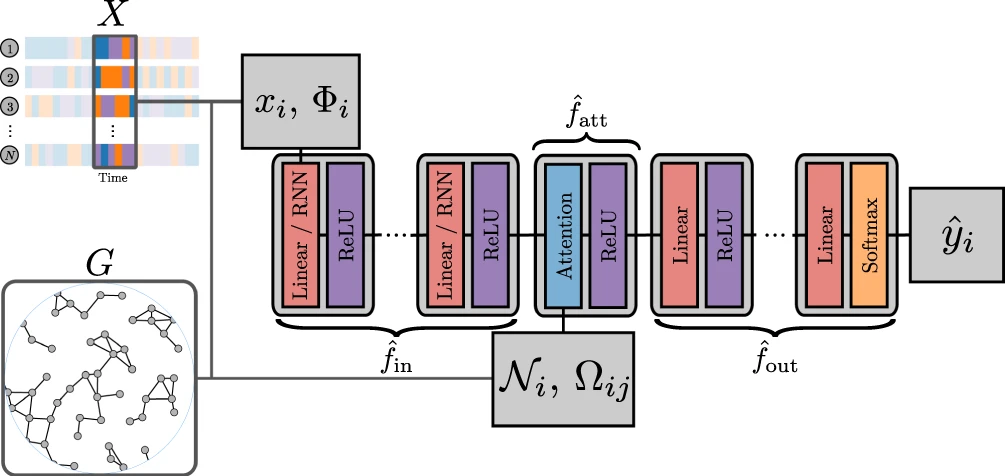
\includegraphics[width=\textwidth]{Figures/chap_exp/GATArch.png}
  \caption[The GAT GNN Architecture]{Schematic showing the layers in the GAT GNN used. Red blocks indicate trainable affine transformations (automorphisms). Purple blocks indicate activation functions. The attention module is in blue and the orange block in the end is the last activation which translates the transformations to the expected format. Image source \cite{murphy}.}
  \label{fig:GATGNN}
\end{figure}

The architecture of the network used can be seen in \fref{fig:GATGNN}.
The state $x_i$ of each node is transformed through a shared MLP
$\hat{f}_{in} : S \rightarrow \mathbb{R}^d$ where $d$ is the resulting
number of node features:
\begin{equation}
  \label{eq:input_layer}
  \xi_i = \hat{f}_{in}(x_i)
\end{equation}
When available, the node attributes $\Phi_i$ are concatenated to $x_i$
so $\hat{f}_{in}: S \times \mathbb{R}^Q \rightarrow \mathbb{R}^d$ and the
$\xi_i$ is now a feature vector with representing the state and attributes of node $v_i$.
The features of the first neighbors are then aggregated using an attention mechanism
discussed in the next section:
\begin{equation}
  \label{eq:first_att}
  v_i = \hat{f}_{att} (\xi_i, \xi_{N_i})
\end{equation}

If available, edge attributes $\Omega_{ij}$ are also included in the attention
mechanism. In a similar manner as before, these attributes are first transformed
into edge features through a $\psi_{ij} = \hat{f}_{edge} (\Omega_{ij})$ where
$\hat{f}_{edge}: \mathbb{R}^P \rightarrow \mathbb{R}^{d_{edge}}$ is also an MLP.
Finally the outcome $\hat{y}_i$ of each node is computed with another MLP $\hat{f}_{out}: \mathbb{R}^d \rightarrow R$:
\begin{equation}
  \label{eq:final_out}
  \hat{y}_i = \hat{f}_{out}(v_i)
\end{equation}

\subsection{Attention Mechanism}
The attention mechanism used is a modified version of the one described by
\citet{velickovic2017graph}. It consists of three trainable functions
$A, B \text{ and} C$ that combine the feature vectors $\xi_i, xi_j \text{ and } \psi_{ij}$ of
pair of connected nodes $v_i$ and $v_j$. The attention coefficient is:
\begin{equation}
  \label{eq:att_coeff}
  \alpha_{ij} = \sigma \big[ A(\xi_i) + B(\xi_j) + C(\psi_{ij}) \big]
\end{equation}
where $\sigma$ is the logistic function which allows for an output range
in $(0, 1)$, 1 meaning maximal influence of $v_j$ on $v_i$ and 0 non-existent influence.
All of the transformations $A, B, \text{ and } C$ are affine and have trainable weights
and biases. 

The aggregation formula is:
\begin{equation}
  \label{eq:att_aggr}
  v_i = \hat{f}_{att}(\xi_i, \xi_{N_i}) = \xi_i + \sum_{v_j \in N_i} \alpha_{ij} \xi_j
\end{equation}
and this $v_i$ contais information about itself and its neighbors through a
multi-head attention mechanism. In contrast with the proposed aggregation mechanism
from the GAT paper, the one used in \eref{eq:att_aggr} uses a general weighted sum
which allows for the architecture to express dynamic process more accurately. The one
used by the GAT paper and other architectures is better when creating models for structure
learning. 

\subsection{Loss Function}
The cross entropy loss function was used in all experiments:
\begin{equation}
  \label{eq:cross_loss}
  L(y_i, \hat{y}_i) = - \sum_m y_{i,m} log \hat{y}_{i,m}
\end{equation}
with $y_i,m$ the $m^{th}$ element of the outcome vector for node $v_i$ a transition
probability vector as discussed before. 

\subsection{Benchmarking and performance}

As a global performance measure, the Pearson correlation coefficient $r$
was used, which in this case is defined on a set of targets $Y$ and predictions $\hat{Y}$:
\begin{equation}
  \label{eq:pearson}
  r = \frac{\mathbb{E}[(Y - \mathbb{E}[Y])(\hat{Y} - E[\hat{Y}])]}{\sqrt{
      \mathbb{E}[(Y - \mathbb{E}[Y])^2]\mathbb{E}[(\hat{Y} - \mathbb{E}[\hat{Y}])^2]}}
\end{equation}

where $\mathbb{E}[Z]$ is the expectation of $Z$. Maximum correlation occurs at
$r=1$ thus $1-r$ can be defined as the global error on a set of target-prediction
pairs.

\section{Experiments}\label{sec:exps}
The experiments conducted for this thesis are largery based on the
methodology and code which was published in the paper ``Deep learning
of contagion dynamics on complex networks'' by \citet{murphy}. The code
which was provided as a supplementary to the publication was modified to
accommodate the scenarios studied. 

\subsection{Generating Data}
Data was generated from two distinct types of graphs, an Erd{\H{o}}s-R{\'e}nyi
$G(n, p)$ model and a ``Barab{\'a}si-Albert'' model, both described in \sref{sec:creating_nw},
where some type of complex dynamics was applied to them. 

For each of these experiments, datasets were created where one type of dynamics
was run on a given network creating at least 1000 samples ?of data, used in
training and validation sets for the Neural Network. Networks and dynamics were
created randomly to avoid using the same training or validation parameters repeatedly;
the starting states for each node were randomized on each run.

Additionally, the maximum likelihood estimators (MLE) were computed
for the transition probabilities of each node with $n_{inf}$ infected
neighbors that transitioned to state $y$ in the dataset, as well as
for all the neighbors. This is stands a reference to benchmark the
accuracy of the model. Finally, the standard deviations of the model's
results are also shown in the figures.


\subsection{SIS}

In this experiment, the SIS model described on \sref{sec:SIS} was used
as a dataset, and the GNN model was trained on that set. The results
are showcased in the figure below for a Barab{\'a}si-Albert network
described in \sref{sec:creating_nw}. Additional results for the same dynamics
run on a $G(n, p)$ network appear in the Appendix on \sref{sec:res_add}.
% Erd{\H{o}}s-R{\'e}nyi (G(n, p))
\begin{figure}[H]
  \centering
  \makebox[\textwidth][c]{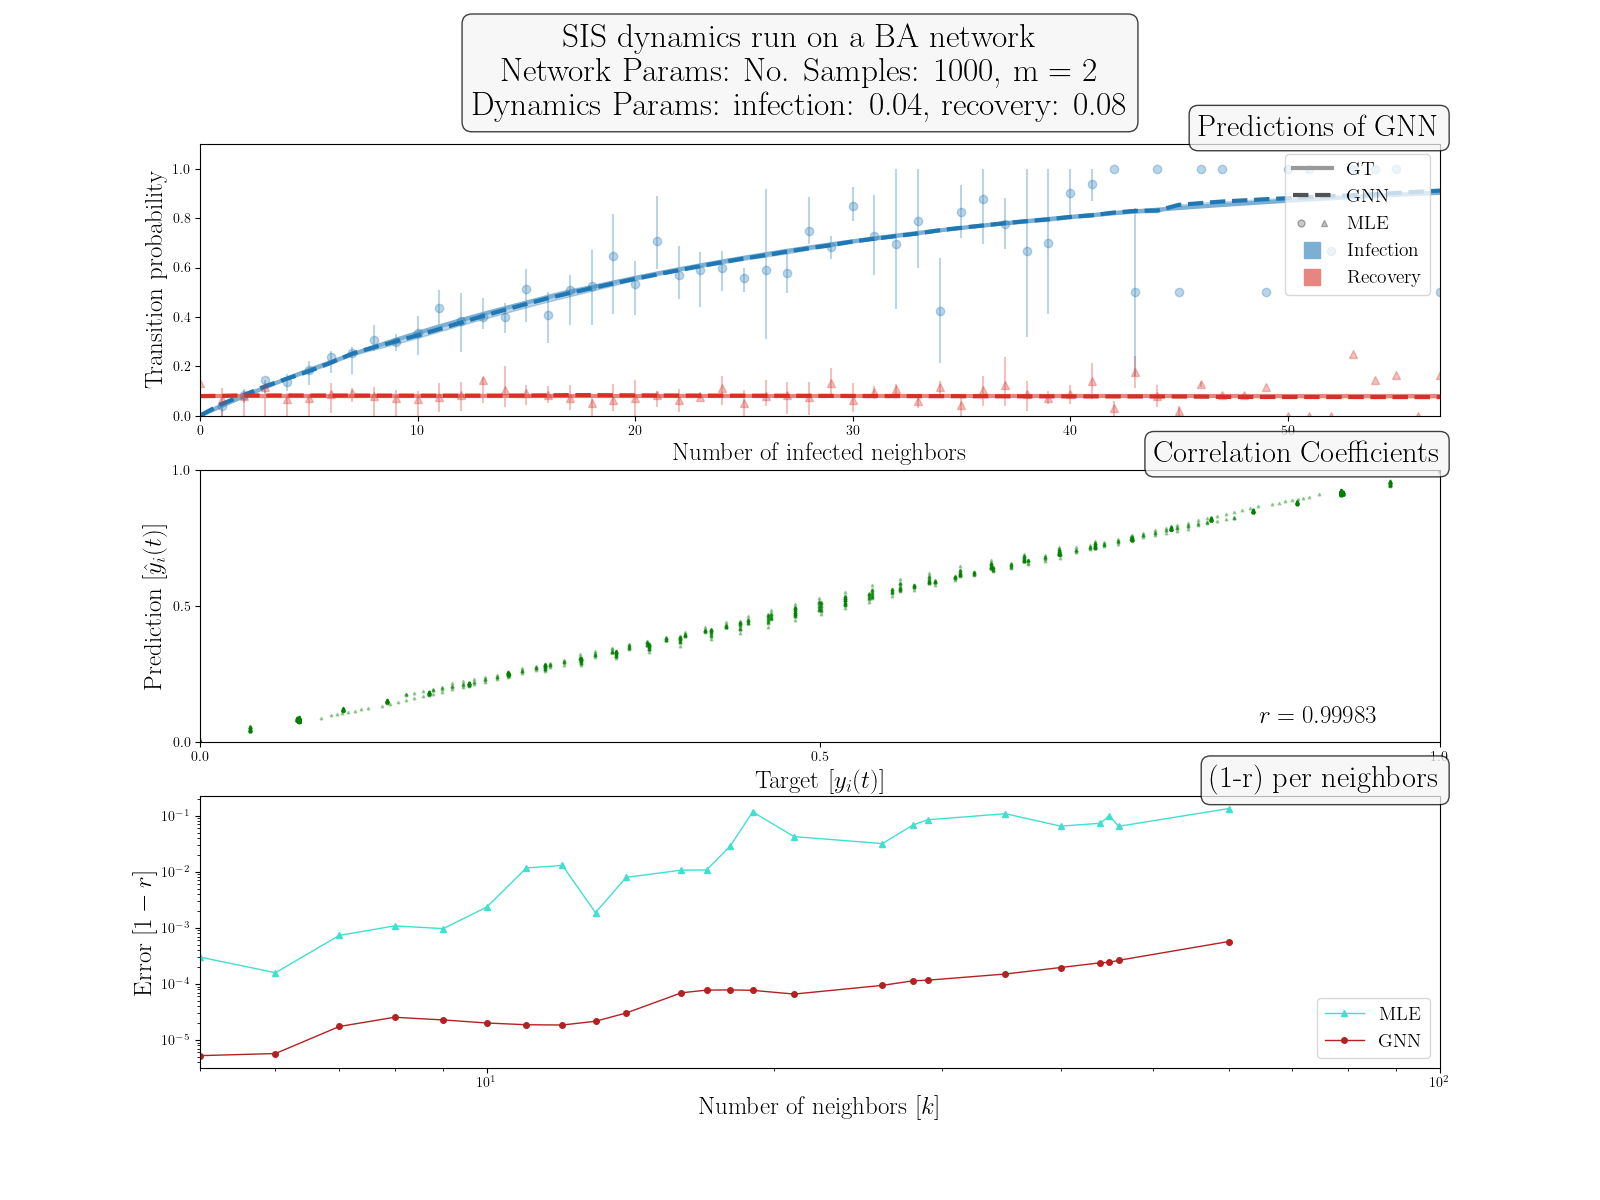
\includegraphics[width=1.4\textwidth]{Figures/chap_exp/ba_sis_default.png}}
  \caption[Results for BA network running SIS dynamics]{
    On the \textbf{top }figure, the transition probabilities for the simple
    contagion dynamics (SIS) dynamics model are shown. \textit{GT} stands
    for ground truth; the transition probabilities used when generating
    the dataset. Circles and triangles represent the MLE computed for said
    probabilities, with circles for the $S \rightarrow I$ transition and
    triangles for $I \rightarrow S$ with error bars present. The colored
    area around the lines is the standard deviation for a given number of
    infected neighbors. On the \textbf{middle} figure, a comparison of
    the predicted and targets ($y_i(t), \hat(y)_i(t)$) appears, with the Pearson
    coefficient $r$ for the whole set of pairs. Each point in this figure represents
    a different pair. On the \textbf{bottom} figure, the errors (1 - $r$) as a function
    of the number of neighbors are presented, both for the GNN and the MLE. These errors
    are computed from the subsets of the prediction and targets pairs where all
    nodes have degree $k$.
  }
  \label{fig:ba_sis}
\end{figure}

\subsection{Planck SIS}

Here, the Planck SIS dynamics described in \sref{sec:planck} were
applied to a BA network. This kind of dynamics presents interest as it
has a complex distribution which is considered more challenging for
both the GNN and MLE to predict accurately.

\begin{figure}[H]
  \centering
  \makebox[\textwidth][c]{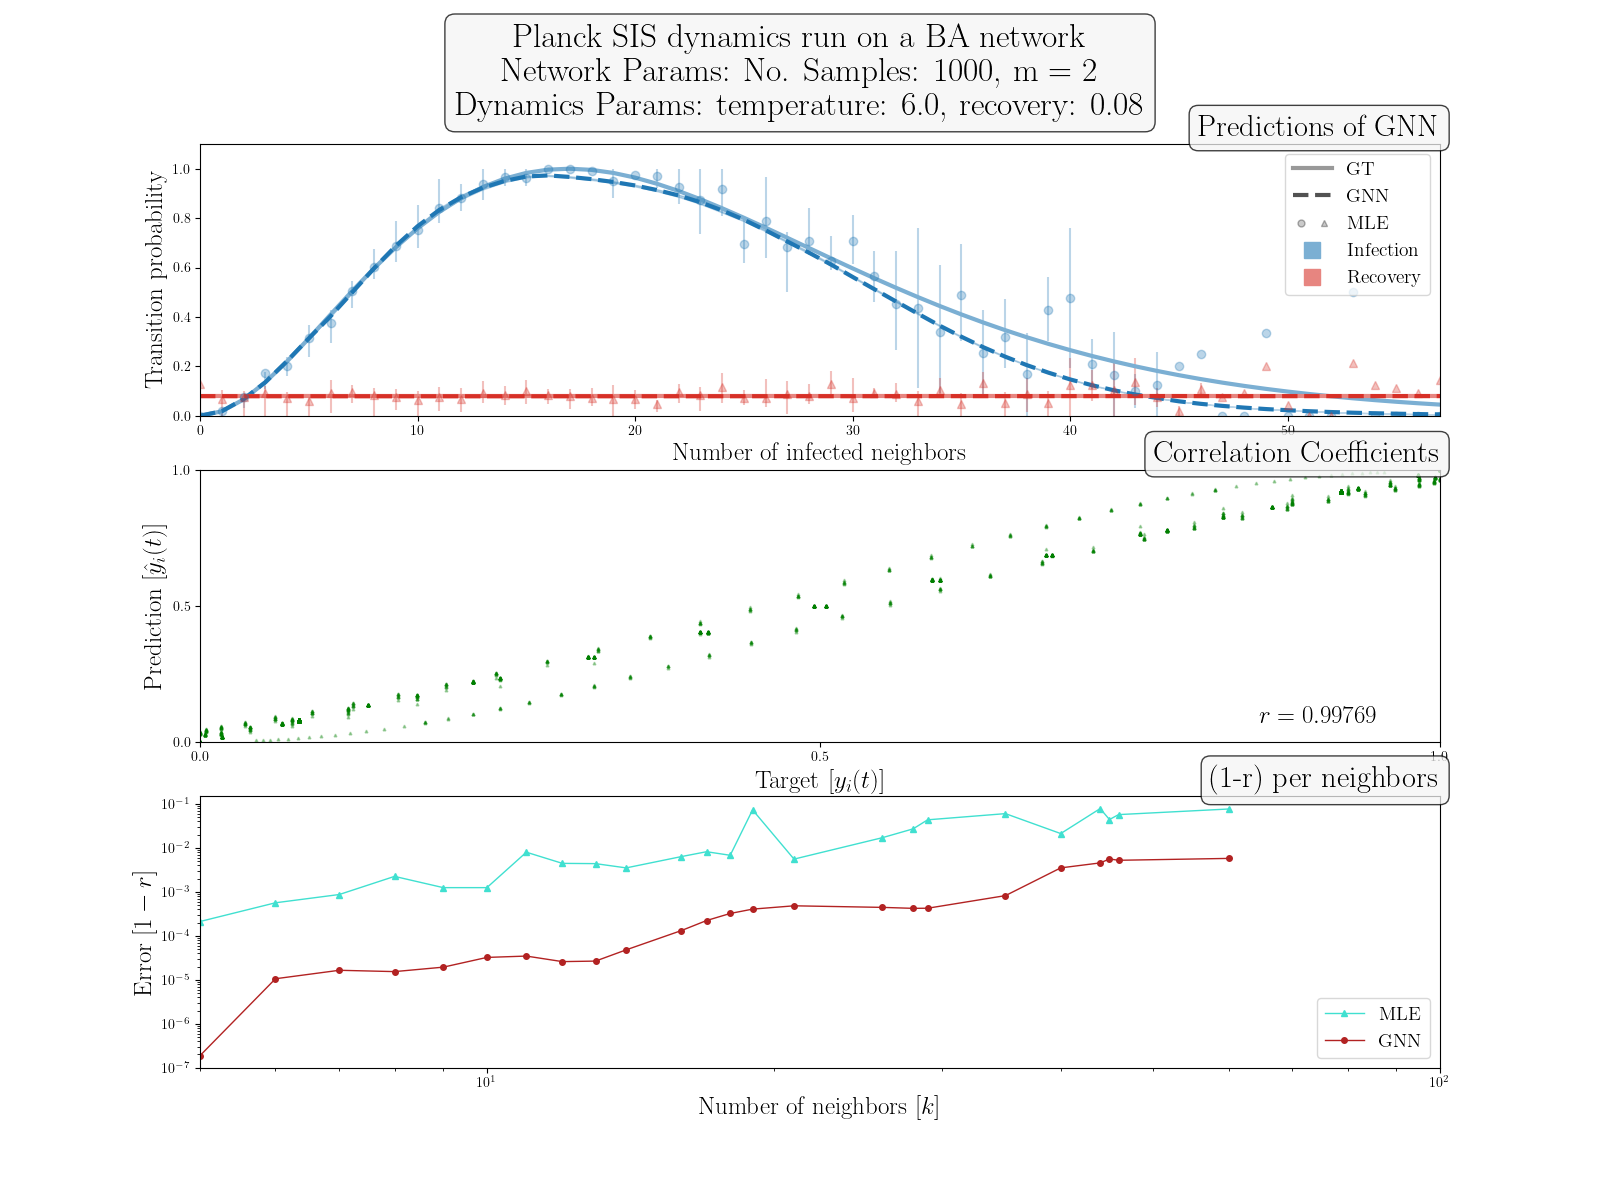
\includegraphics[width=1.4\textwidth]{Figures/chap_exp/ba_plancksis_default.png}}
  \caption[Results for BA network running planck SIS dynamics]{
    Results for Planck SIS dynamics running on a BA
    network. Description same as in \fref{fig:ba_sis}.
  }
  \label{fig:ba_plancksis}
\end{figure}

\newpage
\section{Discussion of results}\label{sec:discussion}

The results indicate that the GNN model is far greater than the MLE,
with the predictions being systematically smoother. The MLE is
computed for each pair of $(x, n_{inf})$ individually, requiring a
large number of pairs for proper accuracy which is rare in realistic
settings.  Even in the synthetic networks used in the approach used
in the experiments, it is especially hard to have pairs of high degree.
It is also impossible for the MLE approach to directly interpolate beyond
the pairs present in the training set where the GNN can, by definition.
Furthermore, during training, the GNN benefits from all samples, small or
high degree, as all of its parameters are always involved during this phase
to improve its predictions leading to smoothness and precision. It is important
to remember than the GNN's goal is to ``learn'' the dynamics of the network,
and is not just a statistical method. 

In the figures \ref{fig:ba_sis}, \ref{fig:ba_plancksis} and \ref{fig:gnp_sis}
the results of the GNN model and MLE are presented. The global performance
of the models was quantified using Pearson's correlation coefficient $r$ for each
pair of predictions and targets $(y(t), \hat{y}(t))$ which is presented in the middle
subfigure. Finally, the error computed as the $1-r$ for each degree
class is showcased in the bottom subfigures and compared to the
equivalent MLE errors. This also allows for a quantification of the
performance of the GNN on each local structure. Furthermore, through this
subfigure, the general accuracy of the GNN over the MLE across all nodes
is straightforward to see. Specifically, as node degree gets larger, the
MLE deteriorates rapidly as a consequence of the scarcity of inputs
of this degree. For the same reason, the MLE is innefective for small
training datasets. The GNN does not suffer from this problem as it uses
every sample to improve its performance as discussed above.
